\documentclass[twocolumn]{aastex631}
\received{\today}
\shorttitle{NEO Follow-up Prioritisation}
\graphicspath{{figures/}}

\usepackage{lipsum}
\usepackage{physics}
\usepackage{multirow}
\usepackage{xspace}
\usepackage{natbib}
\usepackage{fontawesome5}
\usepackage{xcolor}
\usepackage{wrapfig}
\usepackage[figuresright]{rotating}

% remove indents in footnotes
\usepackage[hang,flushmargin]{footmisc} 

\newcommand{\todo}[1]{{\color{red}{[TODO: #1}]}}
\newcommand{\needcite}{{\color{magenta}{(needs citation)}}}
\newcommand{\placeholder}[1]{{\color{gray} \lipsum[#1]}}

% custom function for adding units
\makeatletter
\newcommand{\unit}[1]{%
    \,\mathrm{#1}\checknextarg}
\newcommand{\checknextarg}{\@ifnextchar\bgroup{\gobblenextarg}{}}
\newcommand{\gobblenextarg}[1]{\,\mathrm{#1}\@ifnextchar\bgroup{\gobblenextarg}{}}
\makeatother

\newcommand{\dig}{\texttt{digest2}}
\newcommand{\sss}{S3M}
\newcommand{\mpco}{MPCORB}

\begin{document}

\title{{\large A prioritisation scheme for the follow-up of NEOs}\\\vspace{0.15cm}ASTR 597A Final Project}

% affiliations
\newcommand{\UW}{Department of Astronomy, University of Washington, Seattle, WA, 98195}

\author[0000-0001-6147-5761]{Tom Wagg}
\affiliation{\UW}

\correspondingauthor{Tom Wagg}
\email{tomwagg@uw.edu}

\begin{abstract}
    We present a prioritisation scheme for the follow-up of Near-Earth Objects (NEOs) to prepare for the impact of observations from Rubin Observatory Legacy Survey of Space and Time (LSST). Rubin is expected to vastly increase the rate of detection of candidate NEOs, such that the Near-Earth Object Confirmation Page (NEOCP) will receive 2-3 orders of magnitude more submissions of potential NEOs every night. Many of these objects will attain a perfect \dig{} score of 100 and thus deciding which to prioritise for follow-up would be difficult currently. We use mock LSST observations to quantify the benefits of applying our prioritisation scheme to the NEOCP as an augment to the \dig{} code. We combine the ecliptic latitude, direction of motion relative to the ecliptic plane and the apparent magnitude of objects into a prioritisation score that can be used to differentiate between NEOs and other more numerous background populations (such as main belt asteroids) that receive the same \dig{} score. We find its application would result in 1.5--2x (depending on the capacity for follow-up in a given night) more NEOs receiving follow-up observations each night. This is particularly pertinent for objects that may not remain visible in future nights.
\end{abstract}

\keywords{Near-Earth objects, Asteroids, Solar system, Small Solar System bodies, Surveys}

\section{Introduction}

\begin{figure}[htb]
    \centering
    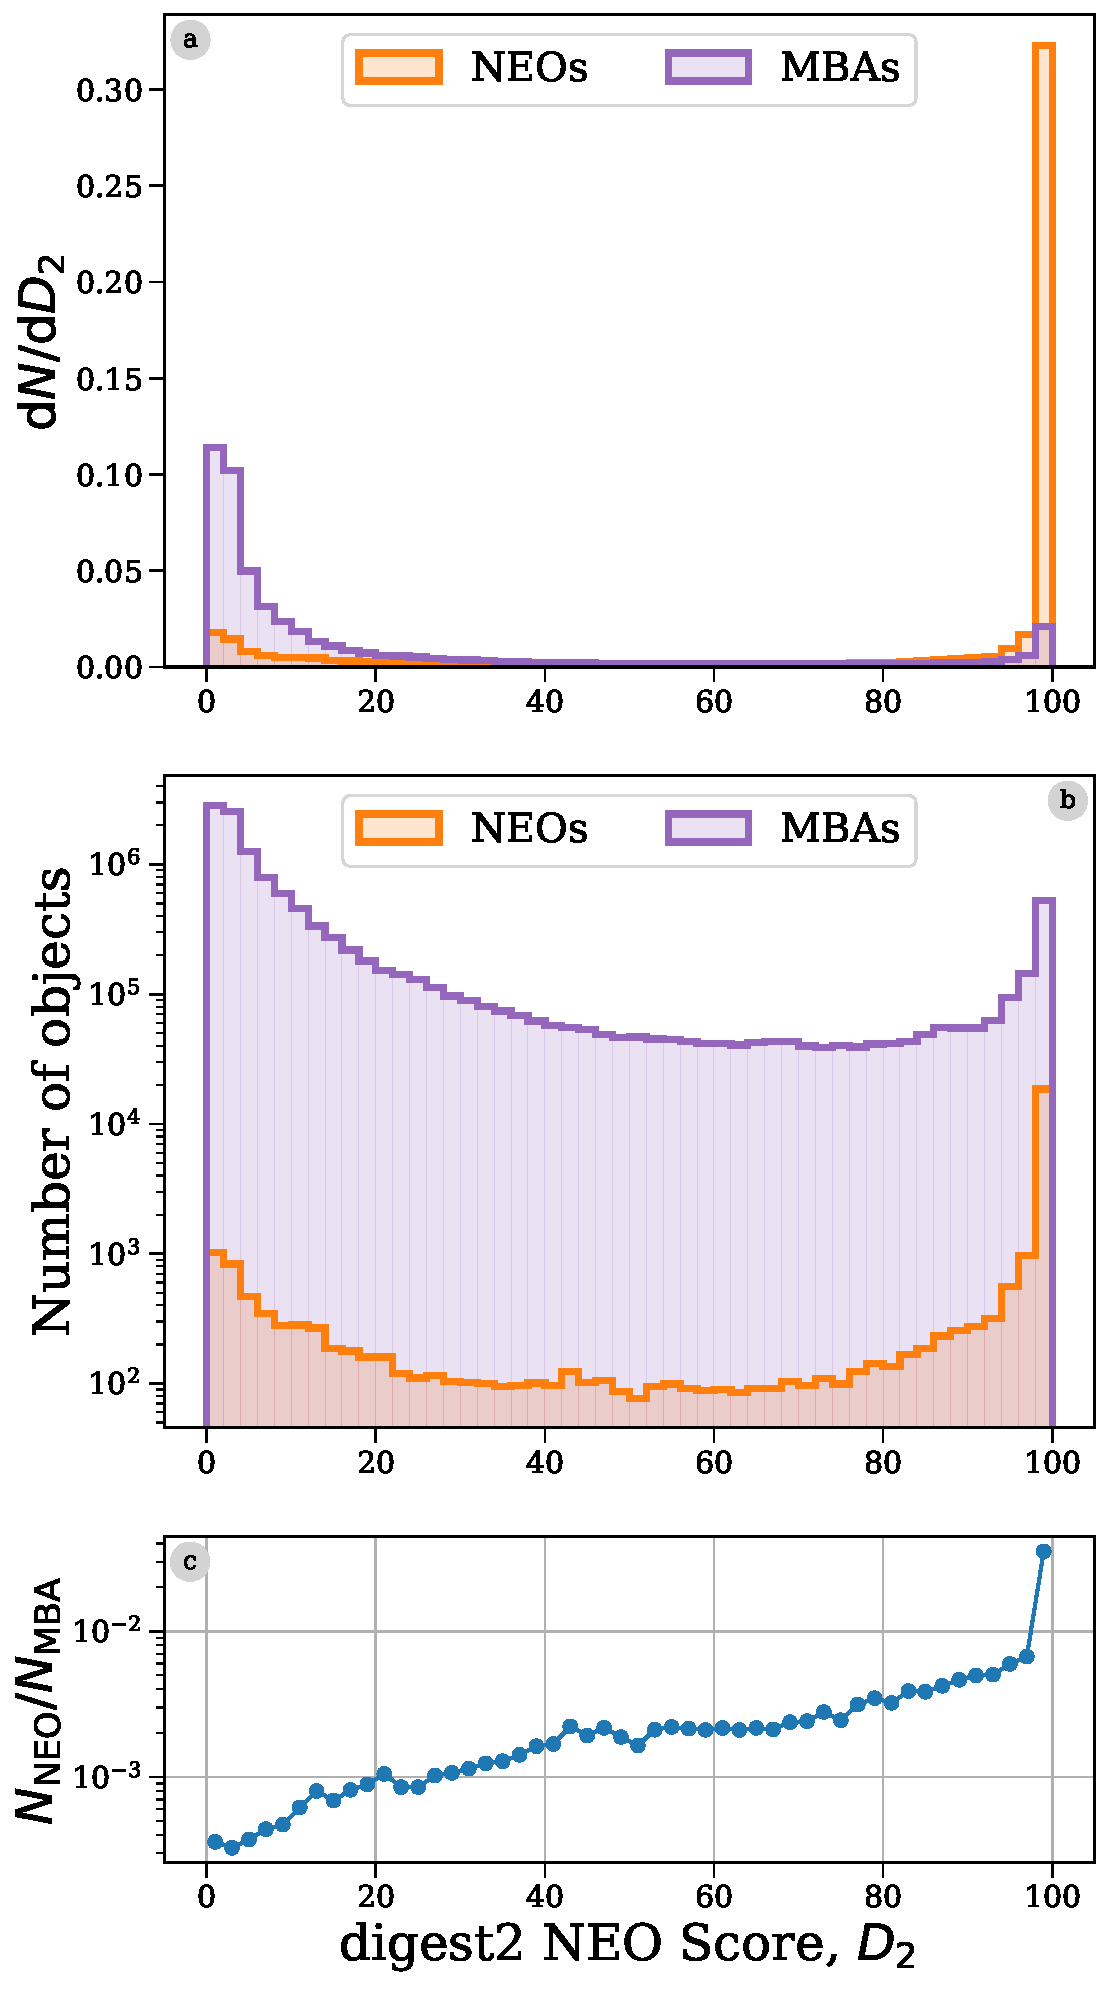
\includegraphics[width=\columnwidth]{digest2_pollution.pdf}
    \caption{\dig{} cannot effectively distinguish NEOs and MBAs with a large MBA background population. \dig{} scores for all NEOs and MBAs observed in the first year of our simulated LSST observations. \textbf{(a)} normalised histograms of \dig{} scores, \textbf{(b)} the same histograms un-normalised \textbf{(c)} ratio of the histograms in (b). Note that the latter two panels are on a logarithmic scale.}
    \label{fig:digest2_should_be_scared}
\end{figure}

Near-Earth Objects (NEOs) are asteroids and comets that have a perihelion distance less than $1.3 \unit{au}$. It is estimated that approximately one fifth of this population passes close enough to Earth that small perturbations in their orbit may lead to intersections with the Earth's orbit and potential collisions \citep[e.g.][]{Jones+2018}. A subset of these objects are known as Potentially Hazardous Asteroids (PHAs), these objects are defined as being at least 140m in diameter that pass within 0.05au of the Earth\footnote{\url{https://cneos.jpl.nasa.gov/about/neo_groups.html}}. PHAs are large enough to make it through the Earth's atmosphere and still cause continent scale damage through impact. Given the threat posed by these objects, a world-wide effort\footnote{E.g.\,\url{https://www.unoosa.org/oosa/en/ourwork/topics/neos/index.html}} has been ongoing to catalogue and determine the orbits and sizes of NEOs including identifying any posing a hazard to the Earth.

The Minor Planet Center maintains a catalogue of known NEOs and their orbits\footnote{\url{https://www.minorplanetcenter.net/iau/MPCORB/NEA.txt}}, as well as the NEO confirmation page (NEOCP\footnote{\url{https://www.minorplanetcenter.net/iau/NEO/toconfirm_tabular.html}}). The NEOCP is a continously updated web page listing newly discovered NEO candidates that should be prioritised for additional observations by the NEO follow-up community. These follow-up observations contribute additional astrometric observations necessary to more accurately determine the orbit of the candidate, as well as photometry to constrain its size. An object is only listed on the NEOCP when it has a high probability of being an NEO. This probability is quantified using the \dig{} code \citep{Keys+2019}. \dig{} assigns a score between 0 and 100 based on potential orbits that fit the observations and only objects with a score of 65 or more are listed on the page. Currently, on average around two dozen objects are added to the NEOCP on each night.

The Rubin Observatory Legacy Survey of Space and Time \citep[LSST,][]{Ivezic+2019} will rapidly increase the rate at which NEO candidates are identified and reported to the NEOCP \citep{sky-is-falling}. \citet{Jones+2018} showed that at the end of the 10-year LSST baseline survey the completeness of NEOs with an absolute magnitude of $H \le 22$ would be 73\%. Most of these objects will be discovered using ``tracklet linking'': a computational technique where at least three pairs of observations (``tracklets'') observed over a 15-night period are identified as belonging to the same object (\citealp{Juric+2017}; Heinze et al., in prep). The orbits of objects discovered with this technique will typically be reasonably well known, and in need of no immediate follow-up. However, this tracklet linking comes at a cost: the object is not identified as interesting until the third tracklet is imaged -- at best, two nights after the first observation or, at worst, nearly two weeks later. This means that potentially interesting (or hazardous) objects may be missed until it's too late to observe (or react to) them.

The number of objects submitted to the NEOCP will increase by several orders of magnitude, and a large fraction of these submissions will be main belt asteriods (MBAs) \citep{sky-is-falling}. This would present difficulties for community follow-up, with too many available candidates (and of low purity) passing the current submission criteria.

\begin{figure}[htb]
    \centering
    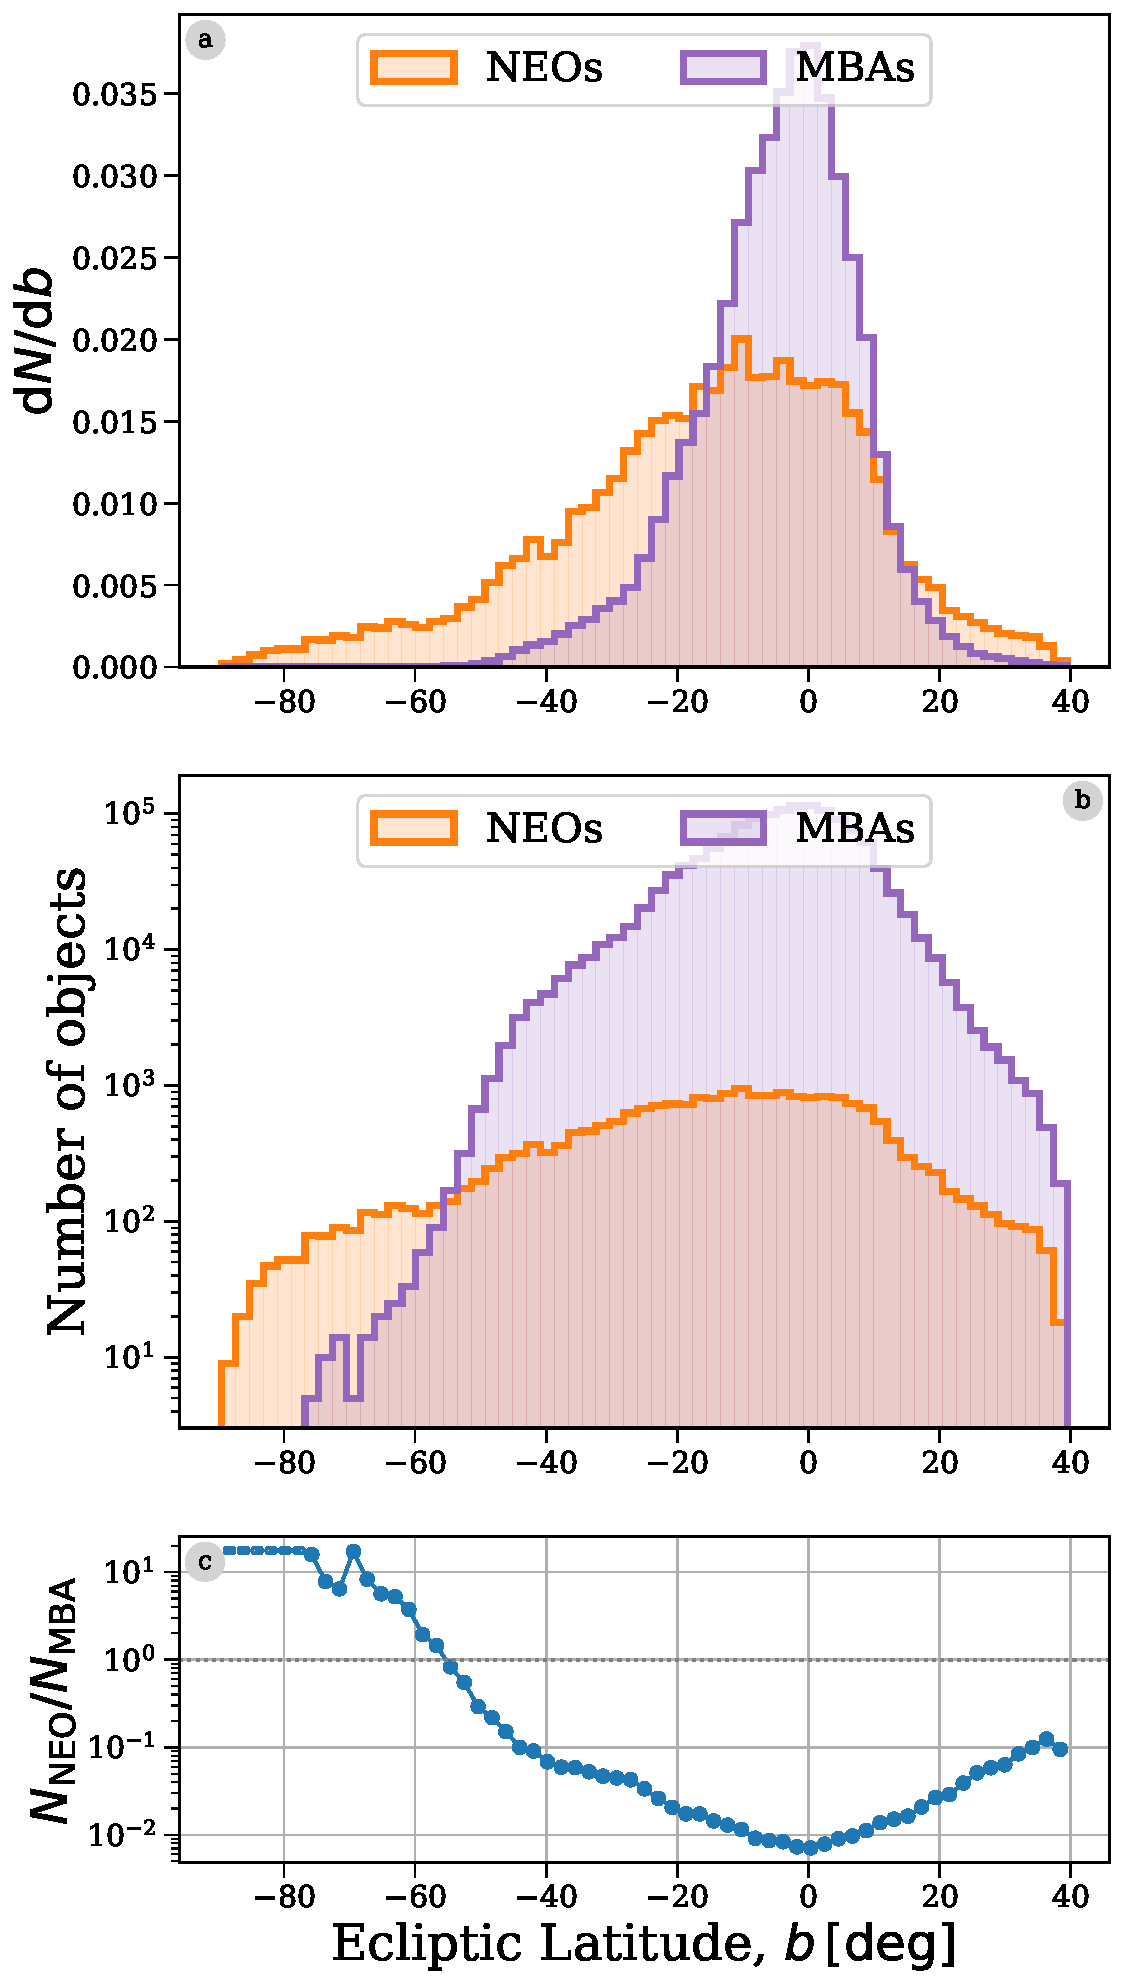
\includegraphics[width=\columnwidth]{figures/ecliptic_latitude_dist_highscore.pdf}
    \caption{MBAs are restricted to low ecliptic latitudes but NEOs more broadly distributed. As Figure~\ref{fig:digest2_should_be_scared}, but for ecliptic latitude and only for observations with a \dig{} score of at least 65.}
    \label{fig:ecl_lat_highscore}
\end{figure}

Due to the vast MBA background, \dig{} performs poorly in identifying NEO candidates, as is demonstrated in Figure~\ref{fig:digest2_should_be_scared}. We show due to the extreme number of MBA submissions, only 1.5\% of submissions meeting the current criteria (a score of least 65) are NEOs, and only 10\% of objects with a perfect score of 100 are actually NEOs. Additionally, a large fraction of objects obtain a score of exactly 100 and it can be difficult to discriminate the best candidates to follow-up among this group. It is clear that this classification scheme requires improvement.
\\

The aim of this paper is to augment \dig{} in classifying NEOs in the presence of a significant MBA background. We simulate one year of LSST observations on a synthetic solar system catalogue and calculate \dig{} scores for each tracklet. We investigate three additional parameters - ecliptic latitude, direction of motion relative to the ecliptic and apparent magnitude - as potential further discriminators between NEOs and MBAs in addition to the \dig{} score. We consider how the combination of these parameters could be used as a sorting metric in order to better identify high probability NEO candidates.

\section{Methods}

\subsection{Simulated tracklet population}

In order to evaluate the efficacy of our priority score, we create a population of simulated tracklets by performing mock LSST observations on a hybrid catalogue of solar system objects that combines synthetic objects with real detections \citep[Appendix A of][]{sky-is-falling,Grav+2011}. We use a modified ``Baseline v2.1''\footnote{\url{https://community.lsst.org/t/survey-simulations-v2-1-april-2022/6538}} 10 year scheduler simulation strategy \citep{Naghib+2019, Cornwall+2020}. These observations account for both scheduled and unscheduled downtime and simulate the current baseline observing strategy that will be followed by LSST. The resulting simulations span 3653 days, and have over 50 million observations. The modification consists of shifting the start of LSST to March 2022, around the epoch of the MPCORB catalogue used to generate the input hybrid catalogue dataset (see Appendix A of \citealp{sky-is-falling}).

We select observations from the simulated LSST dataset that correspond to tracklets. For a tracklet to be built, we require it to satisfy the following criteria:
\begin{enumerate}
    \item \textbf{Number of observations:} We consider only objects with at least 3 observations on a given night.
    \item \textbf{Maximum time separation:} We set the maximum time between observations to 90 minutes.
    \item \textbf{Minimum arc length:} We ensure that each tracklet is at least 1 arcsecond in length.
\end{enumerate}
The motivation behind these cuts is to ensure that the tracklet constrains the on-sky motion of the object sufficiently well, so that its position at a later time can be easily extrapolated. With fewer observations or shorter tracklets, many different orbits could reproduce the same motion on the sky. Moreover, observations that are separated too significantly in time may be spurious linkages, where observations of multiple objects are incorrectly assumed to be of the same source.

\subsection{Parameters included in the priority score}

In addition to the orbital parameters used in computing the \dig{} score, we propose three additional parameters to consider in scoring NEOs: ecliptic latitude, direction of motion relative to the ecliptic plane and apparent magnitude. These parameters are motivated by the fact that MBAs are constrained to lie within the ecliptic plane and around 3au from the Sun, whereas NEOs are often much closer and are not constrained to any location in the ecliptic.

For these reasons, one would predict that an object with a large ecliptic latitude is less likely to be a MBA. For each tracklet, we convert the mean sky position of the observations to an ecliptic latitude, $b$ (and ecliptic longitude, $l$) using \texttt{Astropy} \citep{astropy:2013,astropy:2018,astropy:2022}. In Figure~\ref{fig:ecl_lat_highscore}, we show the distribution of ecliptic latitudes for objects with a \dig{} score of at least 65 (the current threshold for submissions to the NEOCP). As expected, we find that MBAs are concentrated around the ecliptic plane, whereas NEOs extend to the survey limits in either direction. In particular, we note that even without normalising the histogram, NEOs dominate over MBAs below an ecliptic latitude of $-55^{\circ}$.

\begin{figure}[htb]
    \centering
    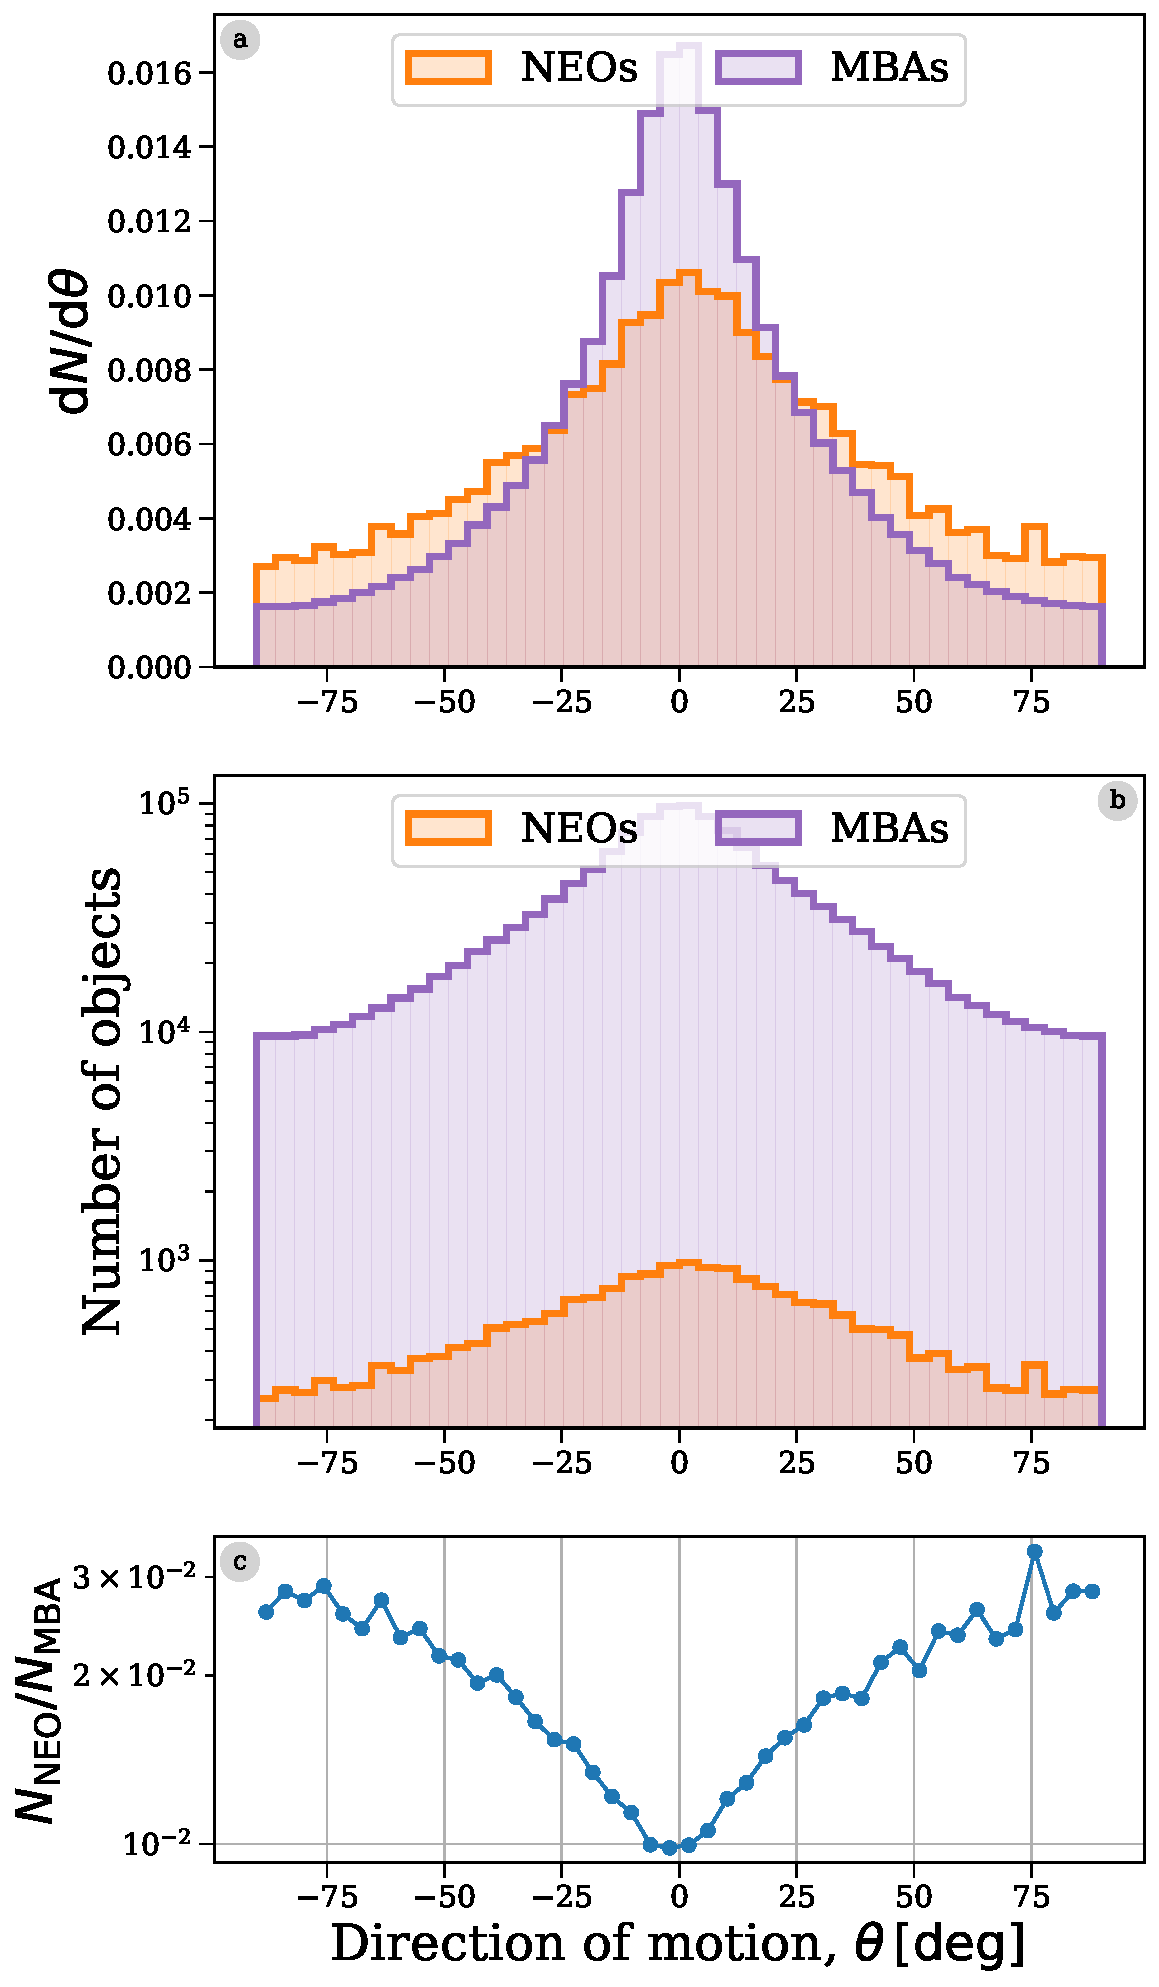
\includegraphics[width=\columnwidth]{figures/direction_dist_highscore.pdf}
    \caption{MBAs are more likely to move along the ecliptic plane than NEOs. As Figure~\ref{fig:digest2_should_be_scared}, but for direction of motion relative to the ecliptic plane and only for observations with a \dig{} score of at least 65.}
    \label{fig:dir_highscore}
\end{figure}

Given that MBAs are constrained to the ecliptic plane and are further away than NEOs, one would predict that their motion is generally along the ecliptic plane, whilst NEOs could move in any direction. To quantify this, we consider the angle of the motion relative to the ecliptic plane
\begin{equation}
    \theta = \arctan \qty( \frac{l_f - l_i}{b_f - b_i} ),
\end{equation}
where $(l_f, b_f)$ are the final ecliptic coordinates of the tracklet and $(l_i, b_i)5$ are the initial ecliptic coordinates of the tracklet. We plot the distributions of $\theta$ in Figure~\ref{fig:dir_highscore}. The separation between NEOs and MBAs in distributions is less clear cut than with the ecliptic latitude but we still find that objects moving away from the ecliptic plane have a larger fraction of NEOs than those moving along the plane.

\begin{figure}[htb]
    \centering
    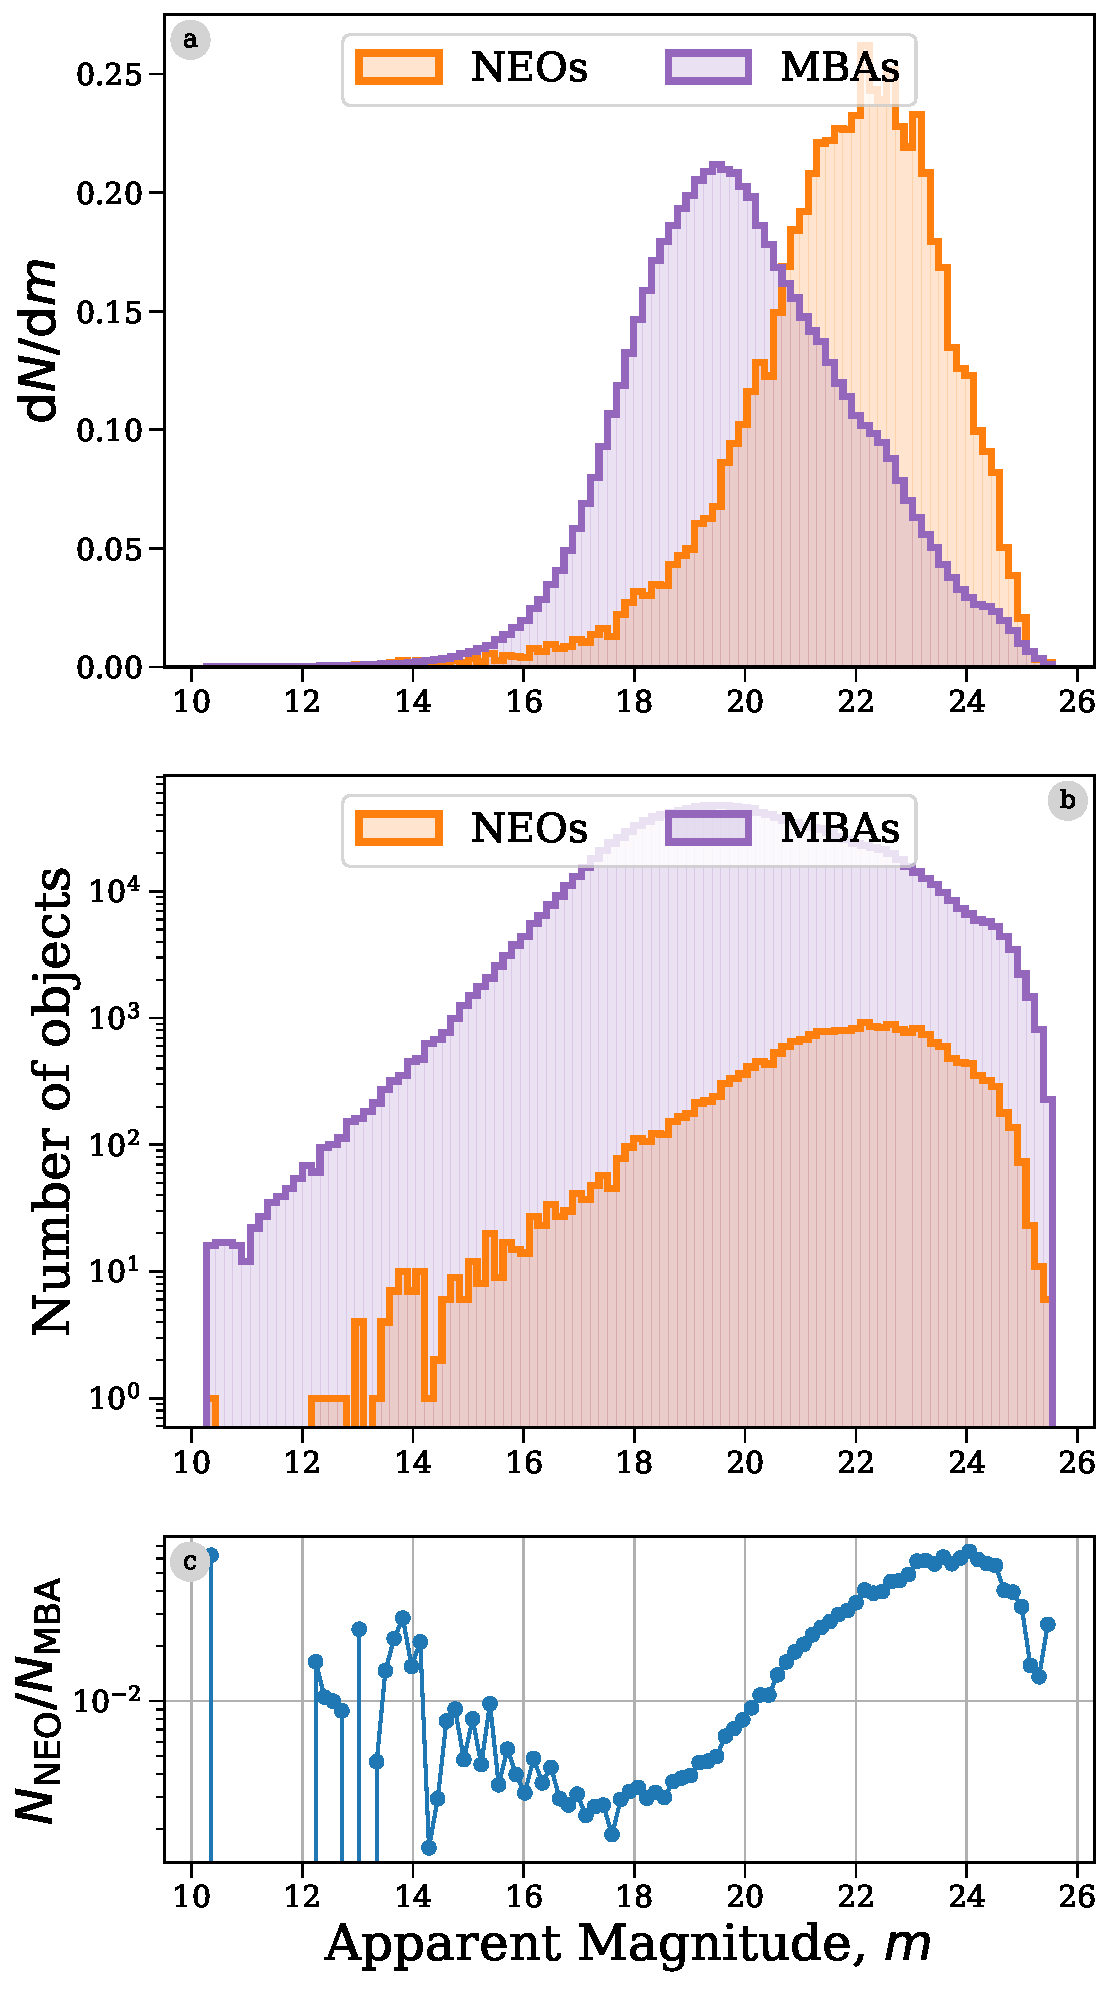
\includegraphics[width=\columnwidth]{figures/apparent_mag_dist_highscore.pdf}
    \caption{NEOs are detectable at fainter apparent magnitudes than MBAs. As Figure~\ref{fig:digest2_should_be_scared}, but for apparent V-band magnitude and only for observations with a \dig{} score of at least 65.}
    \label{fig:app_mag_highscore}
\end{figure}

Lastly, given that NEOs are detected closer to the Earth, one may predict that the faintest NEOs can be detected whilst MBAs of equally faint magnitudes would not be found. We therefore convert the magnitude of each observation from its filter to a V-band magnitude using the colours from \citet{Jones+2018} and assign each tracklet its mean apparent magnitude. In Figure~\ref{fig:app_mag_highscore} we explore the distributions of these magnitudes. As expected, NEOs are peaked at fainter magnitudes than MBAs, but when considering the size of the MBA background (in the lower panels) this difference is not as significant.\clearpage

\subsection{Priority Score Calculation}
\noindent We define the priority score for NEO follow-up as
\begin{equation}
    S \equiv \frac{1}{3} \qty[\frac{|b|}{0.9} + \frac{|\theta|}{0.9} + \frac{(m - m_{\rm min}) \cdot 100}{m_{\rm max} - m_{\rm min}}],
\end{equation}
which results in a score that equally weights the three parameters and has a range of 0 to 100. In the following section we explore the use of this score as an effective sorting metric for the NEOCP.

\section{Results}

Since the \dig{} score cannot exceed 100, a significant fraction of submitted objects will have a perfect score of 100. We find that on average ${\sim}500$ tracklets with at least 3 observations would be submitted to the page and be assigned a score of 100 \emph{per night} in the first year of LSST. Currently the NEOCP is sorted by default by the time at which each object was last updated, and so can be quite random.

Instead of deciding randomly between these objects with perfect scores, it would be more effective to first sort them based on the priority score we have calculated. To investigate this we perform bootstrap sampling on the population of NEOs and MBAs that have scores of 100. We draw 52 NEOs and 468 MBAs for each sample, since these are the average numbers of objects that would be submitted to the NEOCP nightly and attain a score of 100.

For each of these samples we explore the effect of having a randomly ordered list or one sorted by the priority score. Given that the community will not have the capacity to follow-up every candidate given this throughput of objects, we assess how many NEOs would be found when taking only the first $N_{\rm max}$ objects on the list.

\begin{figure}[htb]
    \centering
    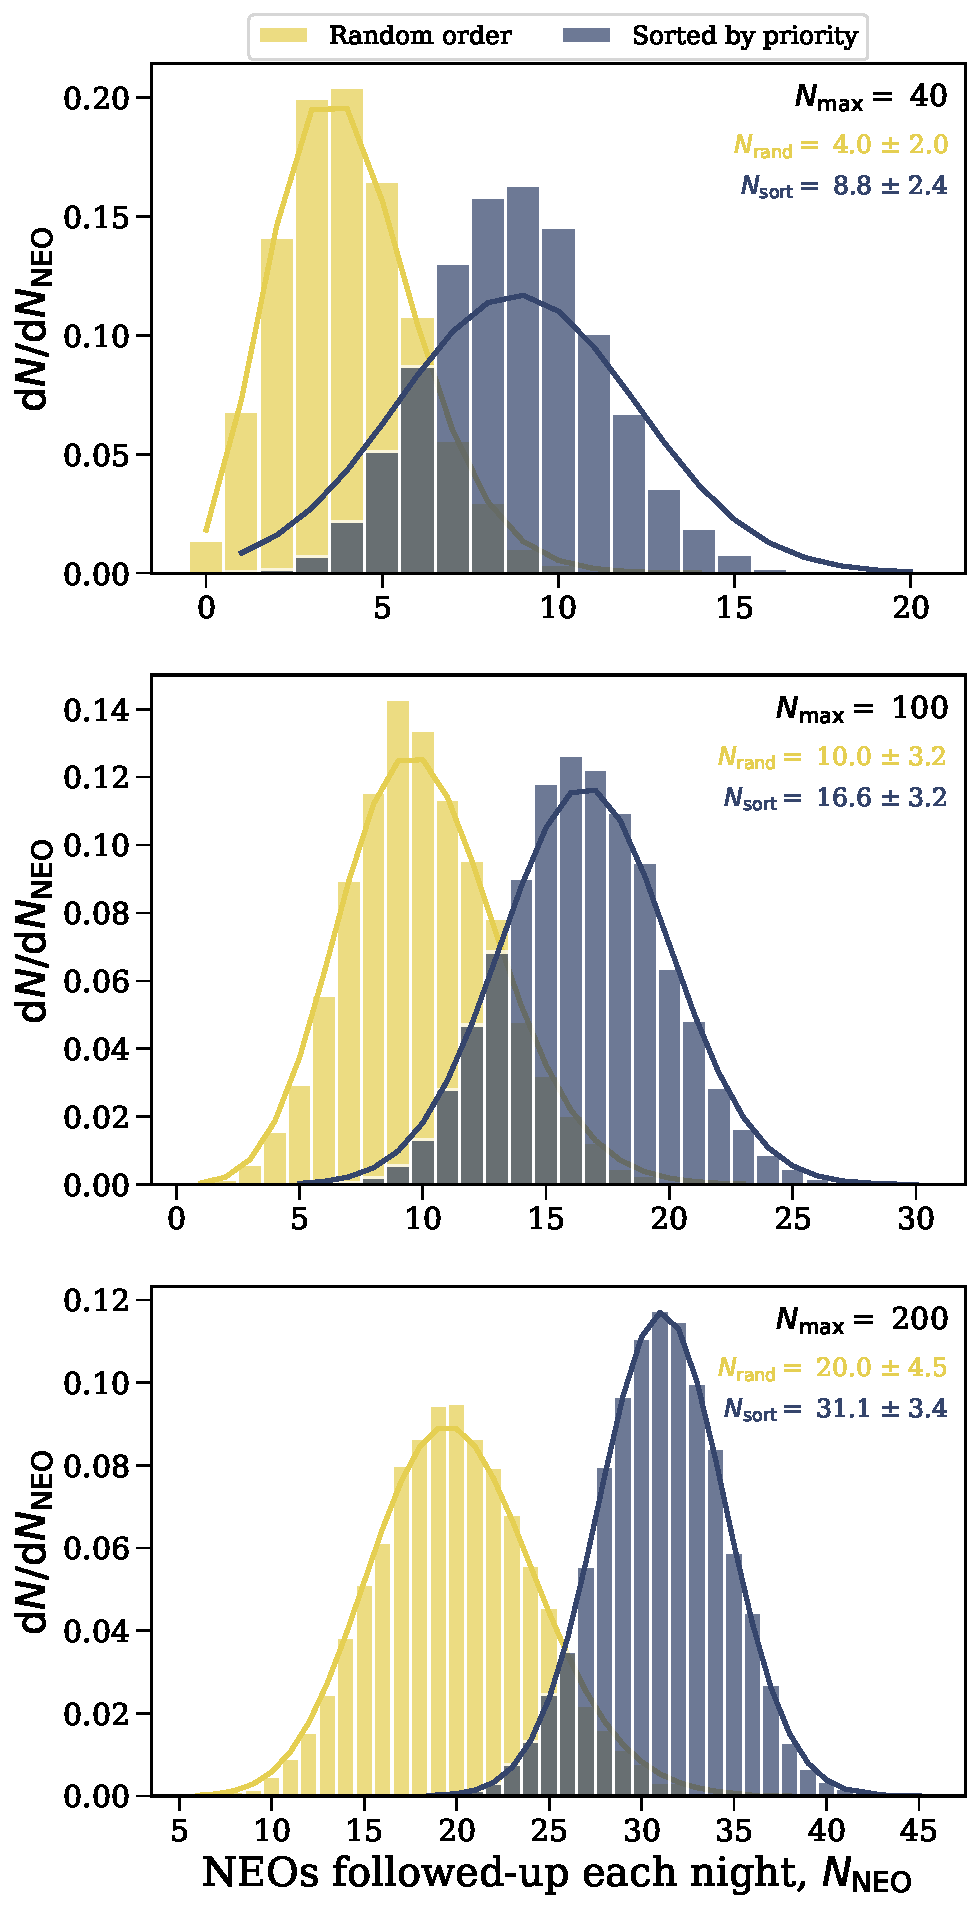
\includegraphics[width=\columnwidth]{sorting_benefits.pdf}
    \caption{Sorting the NEOCP by priority score will increase the number of NEOs receiving follow-up observation by 1.5--2x. Histograms show the average number of NEOs that would be followed-up each night from bootstrapped samples. Each panel corresponds to a different number of maximum follow-ups that could be attempted in a single night and is annotated with the mean number of follow-ups and the standard deviation from the best fit.}
    \label{fig:sort_by_score}
\end{figure}

We show the improvements gained by sorting the list in Figure~\ref{fig:sort_by_score}. From top to bottom we assume values of $40$, $100$ and $200$ for $N_{\rm max}$ and for each distribution we fit for the mean and standard deviation (mostly assuming a Gaussian distribution, except for the distributions centred closer to zero for which we use a Poisson), which we annotate in each panel. In each case we find that sorting the list results in more NEOs being followed-up each night. In particular, assuming an $N_{\rm max}$ of 200 would on average result in 11 more NEOs being follow-up each night, which would mean ${\sim}4000$ additional NEOs would receive follow-up observations.

This improvement is particularly important to consider in cases where the NEO would no longer be visible on a following night - identifying it on that night using our sorting method could make the difference of whether the orbit of the object would be well constrained before it is no longer visible.

We recommend that the NEOCP continue to use \dig{} as a threshold for the page, but use this priority score as a sorting metric for objects that receive the same \dig{} score. Through the joint application of LSST self-follow-up probability algorithm presented in \citep{sky-is-falling} as a further threshold, and this priority score as a sorting metric, we will be able to classify and prioritise NEOs in a significantly more effective manner.

\section{Conclusion}

We present a new prioritisation scheme for NEO follow-up. We performed mock LSST observations and used \dig{} to attain a sample of objects that LSST would send to the NEOCP using the current criteria. We created a new priority score based on ecliptic latitude, direction of motion and apparent magnitude in order to sort the NEOCP and differentiate between objects that attain the same \dig{} score.

We show that sorting the NEOCP by our priority score significantly improves the number of NEOs that receive follow-up observations per night. We find that on average, when assuming a follow-up capacity of 200 objects per night, our sorting metric leads to an additional 11 NEOs receiving follow-up observations, resulting in approximately 4000 more NEOs per year.\\\\\\\\\\\\\\\\\\\\\\\\\\\\\\\\\\\\\\\\\\\\\\\\

\bibliographystyle{aasjournal}
\bibliography{refs}{}

\end{document}